\section{Section 4: Leslie Matrix Model}
\subsection{Background}

\begin{frame}{Limitations of previous models}
\begin{itemize}
    \item So far, our models (Malthusian, Logistic) assumed all individuals in a population are identical.
    \item \textbf{In reality, age matters:}
    \begin{itemize}
        \item \textbf{Reproduction:} Young individuals (larvae, babies) cannot reproduce yet.
        \item \textbf{Survival:} Survival rates often depend on age (e.g., higher mortality in very young or very old individuals).
    \end{itemize}
    \vspace{1em}
    \item To capture this, we need an \textbf{age-structured model}.
    \item The most common discrete-time model for this is the \textbf{Leslie Matrix}.
\end{itemize}
\end{frame}

\begin{frame}{The Leslie Matrix Model}
\small
Developed by Patrick H. Leslie in 1945.
\vspace{1em}
\begin{itemize}
    \item It tracks the number of females in different age classes at discrete time steps.
    \item \textbf{Variables:}
    \begin{itemize}
        \item $n_i(t)$: Number of individuals in age class $i$ at time $t$.
        \item $F_i$: \textbf{Fecundity} (fertility) rate. Average number of female offspring produced by a female in age class $i$.
        \item $S_i$: \textbf{Survival} rate. Probability that a female in age class $i$ survives to age class $i+1$.
    \end{itemize}
\end{itemize}
\end{frame}

\begin{frame}{Mathematical Formulation}
\footnotesize
If we have 3 age classes, the population vector at time $t+1$ is calculated as:

\begin{align*}
    n_1(t+1) &= F_1 n_1(t) + F_2 n_2(t) + F_3 n_3(t) && \text{\textbf{New offspring} (born from all classes)} \\
    n_2(t+1) &= S_1 n_1(t) && \text{\textbf{Survivors} from class 1 moving to 2} \\
    n_3(t+1) &= S_2 n_2(t) && \text{\textbf{Survivors} from class 2 moving to 3}
\end{align*}

\vspace{1em}
This can be written in matrix form:
\begin{equation*}
\begin{bmatrix} n_1 \\ n_2 \\ n_3 \end{bmatrix}_{t+1} = 
\begin{bmatrix}
F_1 & F_2 & F_3 \\
S_1 & 0 & 0 \\
0 & S_2 & 0
\end{bmatrix}
\begin{bmatrix} n_1 \\ n_2 \\ n_3 \end{bmatrix}_t
\end{equation*}

\begin{equation*}
    \mathbf{n}_{t+1} = \mathbf{L} \cdot \mathbf{n}_t
\end{equation*}

\end{frame}

\begin{frame}{Life Cycle with Age-Class Structure}
    % Introductory text
    \small
    Individuals are grouped into discrete age classes of equal duration.
    
    \vspace{1em}
    
    % TikZ Diagram Reproduction
    \begin{center}
    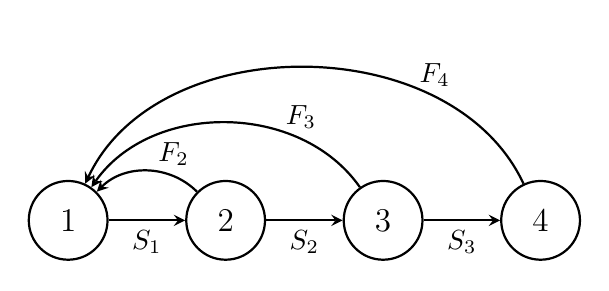
\begin{tikzpicture}[
        scale=1, 
        transform shape, 
        >=stealth, % Arrow tip style
        node distance=2.0cm, 
        thick, 
        main/.style={circle, draw, minimum size=1.0cm, font=\large}
    ]

        % Nodes (Circles representing Age Classes)
        \node[main] (1) {1};
        \node[main] (2) [right of=1] {2};
        \node[main] (3) [right of=2] {3};
        \node[main] (4) [right of=3] {4};

        % Survival Arrows (Straight, below)
        \path[->] 
            (1) edge node[below] {$S_1$} (2)
            (2) edge node[below] {$S_2$} (3)
            (3) edge node[below] {$S_3$} (4);

        % Fecundity/Birth Arrows (Curved, above)
        % Note: "bend right" curves UP when moving from Right to Left
        \path[->] 
            (2) edge[bend right=45] node[above, near start] {$F_2$} (1)
            (3) edge[bend right=55] node[above, near start] {$F_3$} (1)
            (4) edge[bend right=65] node[above, near start] {$F_4$} (1);

    \end{tikzpicture}
    \end{center}

    \vspace{0.5em}

    % Explanatory Text
    \footnotesize
    \begin{itemize}
        \item \textbf{Circles:} Represent specific age classes or ages (1 to 4).
        \item \textbf{Horizontal Arrows ($S_x$):} Represent \textbf{survival probabilities}. Probability that an individual of age $x$ survives to age $x+1$. There is no survival beyonf group 4.
        \item \textbf{Curved Arrows ($F_x$):} Represent \textbf{births (fecundity)}. Arrows lead back to Age 1 because newborns enter the first class. Arrows emerging from ages 2, 3, and 4 indicate these ages are reproductive.
    \end{itemize}
\end{frame}


\begin{frame}{Matrix Representation of the Life Cycle}
    \small
    The life cycle diagram translates directly into a \textbf{projection matrix} (Leslie Matrix).
    
    \vspace{1em}


            \textbf{The Equation:}
            \begin{equation*}
                \mathbf{n}_{t+1} = \mathbf{L} \cdot \mathbf{n}_t
            \end{equation*}
            
            \vspace{0.5em}
            
            \textbf{The Matrix Expansion:}
            \begin{equation*}
            \begin{bmatrix} n_1 \\ n_2 \\ n_3 \\ n_4 \end{bmatrix}_{t+1}
            =
            \begin{bmatrix}
                0 & F_2 & F_3 & F_4 \\
                S_1 & 0 & 0 & 0 \\
                0 & S_2 & 0 & 0 \\
                0 & 0 & S_3 & 0
            \end{bmatrix}
            \begin{bmatrix} n_1 \\ n_2 \\ n_3 \\ n_4 \end{bmatrix}_{t}
            \end{equation*}

\end{frame}

\begin{frame}{Structure of the Leslie Matrix}
\begin{center}
    \LARGE
    $
    \mathbf{L} = 
    \begin{bmatrix}
    F_1 & F_2 & F_3 & \dots & F_k \\
    S_1 & 0 & 0 & \dots & 0 \\
    0 & S_2 & 0 & \dots & 0 \\
    \vdots & \vdots & \ddots & \dots & \vdots \\
    0 & 0 & \dots & S_{k-1} & 0
    \end{bmatrix}
    $
\end{center}
\vspace{1em}
\small
\begin{itemize}
    \item \textbf{Top Row:} Fertility rates (production of new offspring).
    \item \textbf{Sub-diagonal:} Survival rates (transition to next age group).
    \item \textbf{All other entries:} Zero (you cannot skip an age or get younger).
\end{itemize}
\end{frame}

\begin{frame}{Long-term Dynamics}
What happens if we simulate this for many time steps?
\vspace{1em}
\begin{itemize}
    \item \textbf{Population Growth:} The total population eventually grows (or declines) at a constant rate $\lambda$.
    \item \textbf{Stable Age Distribution:} The \textit{proportion} of individuals in each age class becomes constant.
    \begin{itemize}
        \item Example: 60\% juveniles, 30\% adults, 10\% seniors.
        \item This happens regardless of the initial population state!
    \end{itemize}
\end{itemize}
\vspace{1em}
\textit{Note for linear algebra enthusiasts: $\lambda$ is the dominant eigenvalue of $L$, and the stable age distribution is the corresponding eigenvector.}
\end{frame}


\subsection{Population Growth Rate ($\lambda$)}

\begin{frame}{The Finite Rate of Increase ($\lambda$)}
    \small
    As the population approaches the Stable Age Distribution, it begins to grow (or decline) at a constant rate every time step.
    
    \vspace{1em}
    We call this rate $\lambda$ (lambda).
    
    \begin{equation*}
        N_{total}(t+1) = \lambda \cdot N_{total}(t)
    \end{equation*}
    
    \vspace{1em}
    \textbf{Biological Interpretation:}
    \begin{itemize}
        \item \textbf{$\lambda > 1$:} The population is \textbf{growing} exponentially.
        \item \textbf{$\lambda = 1$:} The population is \textbf{stable} (stationary).
        \item \textbf{$\lambda < 1$:} The population is \textbf{declining} to extinction.
    \end{itemize}
\end{frame}

\begin{frame}{Importance of $\lambda$}
    Why is calculating $\lambda$ so critical in conservation and ecology?
    \vspace{1em}
    \begin{itemize}
        \item \textbf{Conservation Status:} Determines if an endangered species is recovering ($\lambda > 1$) or needs intervention ($\lambda < 1$).
        \item \textbf{Pest Control:} To eradicate a pest, we must lower survival/fertility until $\lambda < 1$.
        \item \textbf{Harvesting:} In fisheries or forestry, we want to harvest the "excess" without driving $\lambda$ below 1.
        \item \textbf{Comparative Analysis:} Allows us to compare population health across different habitats regardless of current population size.
    \end{itemize}
\end{frame}

\begin{frame}{How to Calculate $\lambda$}
    There are two main ways to find $\lambda$:
    
    \vspace{1em}
    \textbf{1. The Analytical Method (Eigenvalues)}
    \begin{itemize}
        \item $\lambda$ is the \textbf{dominant eigenvalue} (largest absolute value) of the Leslie Matrix $\mathbf{L}$.
        \item Requires linear algebra: $\det(\mathbf{L} - \lambda \mathbf{I}) = 0$.
    \end{itemize}
    
    \vspace{1em}
    \textbf{2. The Numerical Method (Simulation)}
    \begin{itemize}
        \item If we simulate the population long enough, the ratio between consecutive years converges to $\lambda$.
        \item $\lambda \approx \frac{N(t+1)}{N(t)}$ (for large $t$).
    \end{itemize}
\end{frame}


\subsection{Exercise}

\begin{frame}{Task 4.1: Defining the Model}
\textbf{Scenario: A population of hypothetical birds}
\begin{itemize}
    \item \textbf{Class 1 (Chicks, 0-1 yr):} Do not reproduce ($F_1=0$). 60\% survive to next year ($S_1=0.6$).
    \item \textbf{Class 2 (Young Adults, 1-2 yr):} Moderate reproduction ($F_2=1.5$). 50\% survive ($S_2=0.5$).
    \item \textbf{Class 3 (Older Adults, 2-3 yr):} High reproduction ($F_3=2.0$). They die after this year ($S_3=0$).
\end{itemize}
\vspace{1em}
\textbf{Your Task:}
\begin{enumerate}
    \item Construct the Leslie Matrix $L$ in Python (using NumPy).
    \item Define an initial population vector $n_0$: 100 chicks, 0 adults.
\end{enumerate}
\end{frame}

\begin{frame}[fragile]{Solution 4.1: Defining the Model}
\small
\begin{lstlisting}[language=Python]
import numpy as np

# Define parameters
F1 = 0;   F2 = 1.5; F3 = 2.0
S1 = 0.6; S2 = 0.5

# Construct Leslie Matrix
L = np.array([[F1, F2, F3],
              [S1, 0,  0],
              [0,  S2, 0]])

# Initial population (100 chicks, 0 young adults, 0 old adults)
n0 = np.array([100, 0, 0])
\end{lstlisting}
\end{frame}

\begin{frame}{Task 4.2: Simulation Loop}
\textbf{Your Task:}
\begin{itemize}
    \item Simulate the population for 20 years.
    \item Store the population vector for each year.
    \item \textit{Hint: You will need a matrix to store results, where columns represent time steps.}
\end{itemize}
\end{frame}

\begin{frame}[fragile]{Solution 4.2: Simulation Loop}
\small
\begin{lstlisting}[language=Python]
years = 20
# Pre-allocate matrix (3 rows, years+1 columns)
pop_history = np.zeros((3, years + 1))

# Set initial year (Python is 0-indexed)
pop_history[:, 0] = n0

# Loop through time
for t in range(years):
    # n(t+1) = L @ n(t)
    # The @ operator performs matrix multiplication
    pop_history[:, t+1] = L @ pop_history[:, t]
\end{lstlisting}
\end{frame}

\begin{frame}{Task 4.3: Analyzing Results}
\textbf{Your Task:}
\begin{enumerate}
    \item Calculate the \textbf{total population} for each year (sum of all age classes).
    \item Plot the Total Population over time.
    \item Plot the specific age classes over time.
\end{enumerate}
\end{frame}

\begin{frame}[fragile]{Solution 4.3: Plotting}
\tiny
\begin{lstlisting}[language=Python]
import matplotlib.pyplot as plt

# Calculate total population (sum each column, axis=0)
total_pop = np.sum(pop_history, axis=0)
t = np.arange(years + 1)

# Plot
plt.figure(figsize=(10, 6))

plt.subplot(2,1,1)
plt.plot(t, total_pop, 'k-', linewidth=2)
plt.title('Total Population Growth'); plt.grid(True)

plt.subplot(2,1,2)
plt.plot(t, pop_history[0, :], 'b-o', label='Chicks')
plt.plot(t, pop_history[1, :], 'r-o', label='Young')
plt.plot(t, pop_history[2, :], 'g-o', label='Old')
plt.legend(); plt.grid(True)
plt.show()
\end{lstlisting}
\end{frame}

\begin{frame}{Task 4.4: Stable Age Distribution (Advanced)}
We claimed earlier that the \textit{proportion} of age groups becomes constant.
\vspace{1em}
\textbf{Your Task:}
\begin{itemize}
    \item Normalize the population data at each step (divide each column by the total population of that column).
    \item Inspect the last few columns of this normalized matrix.
    \item Are the proportions changing?
\end{itemize}
\end{frame}

\begin{frame}[fragile]{Solution 4.4: Stable Age Distribution}
\small
\begin{lstlisting}[language=Python]
# Normalize to find proportions
# axis=0 means we sum down the columns
proportions = pop_history / np.sum(pop_history, axis=0)

# Display the proportions for the last year (-1 index)
print("Final Age Distribution:")
print(proportions[:, -1])

# Check the previous year to see if it stabilized
print("Previous Year Distribution:")
print(proportions[:, -2])
\end{lstlisting}

\vfill
\textit{You should see that the vector values stabilize, confirming the Stable Age Distribution theorem.}
\end{frame}

\begin{frame}{Task 4.5: Calculating $\lambda$ in Python}
    \textbf{Your Task:}
    \begin{enumerate}
        \item \textbf{Method A (Simulation):} Calculate the growth rate using the total population from the \textit{last two years} of your simulation.
        $$ \lambda_{sim} = \frac{\text{Total Pop (Year 20)}}{\text{Total Pop (Year 19)}} $$
        
        \item \textbf{Method B (Linear Algebra):} Use NumPy's linear algebra library to calculate the eigenvalues of matrix $L$ directly.
        \item Compare the two values.
    \end{enumerate}
\end{frame}

\begin{frame}[fragile]{Solution 4.5: Calculating $\lambda$}
\small
\begin{lstlisting}[language=Python]
# --- Method A: From Simulation ---
# Total population at last step / Total population at 2nd to last step
lambda_sim = total_pop[-1] / total_pop[-2]
print(f"Simulated Lambda: {lambda_sim:.4f}")

# --- Method B: Eigenanalysis ---
# Calculate eigenvalues
eigenvalues = np.linalg.eigvals(L)

# The dominant eigenvalue is the maximum real value
lambda_eig = np.max(np.real(eigenvalues))
print(f"Theoretical Lambda: {lambda_eig:.4f}")

# They should be nearly identical!
\end{lstlisting}
\vspace{1em}
\footnotesize
\textit{Note: `np.linalg.eigvals` returns complex numbers. We use `np.real` and `np.max` to find the dominant growth rate.}
\end{frame}